\documentclass[a4paper,12p]{article}
\usepackage[utf8]{inputenc}
\usepackage[ngerman]{babel}
\usepackage[a4paper, left=2.5cm, right=2.5cm]{geometry}
\usepackage{amsmath}
\usepackage{tikz}
\usepackage{graphicx}
\usepackage{mathtools}
\usepackage{cancel}
\usepackage{amssymb}


\title{\huge Modellbildung\\\large \huge Beispielsammlung}
\author{\huge 4.Semester ET-Studium}
\date{\huge Oktober 2019}

\begin{document}

	\maketitle
	\newpage
	\tableofcontents
	\newpage
	
	\section{Einleitung}
	In dieser Ausarbeitung befinden sich sämtliche Rechenwege der Modellbildungsprüfung beginnend ab dem Jahr 2015. Die Angaben zu den hier ausgearbeiteten Prüfungen befinden sich auf der Homepage des ACIN. Sämtlichen verwendeten Formeln befinden sich in der Formelsammlung, welche ebenfalls auf der Homepage des ACIN zu finden ist. Ich hoffe dieses Dokument hilft euch weiter. 
	
	\section{Prüfungen}
	
	\subsection{26.06.2015}
	\textbf{Beispiel 1} \\ \\
a)\\ \\
Die generalisierten Koordinaten lauten
\[
	\textbf{q} = \left[ \begin{matrix}
		\varphi \\
		\psi
	\end{matrix}\right]
\]
Diese beiden sind deswegen die geeigneten generalisierten Koordinaten, weil diese sich mit der Zeit ändern können. \\ 
Die beiden Ortsvektoren $\textbf{r}_2$ und $\textbf{r}_K$ werden direkt aus Angabe abgelesen.
\[
	\textbf{r}_2 = \left[\begin{matrix}
		\frac{1}{2} L_2 + L_1 \sin\varphi \\
		-L_1\cos\varphi
	\end{matrix}\right] , 
	\textbf{r}_K = \left[\begin{matrix}
		\frac{1}{2} L_2 + L_1\sin\varphi + l\sin\psi \\
		-L_1\cos\varphi - l\cos\psi
	\end{matrix}\right]
\]
b) \\ \\
Den translatorische Geschwindigkeitsvektor erhält man durch die zeitliche Ableitung des entsprechenden Ortsvektors.
\[
	\dot{\textbf{r}}_K = \underbrace{L_1\dot{\varphi}\left[\begin{matrix}
		\cos\varphi \\
		\sin\varphi
	\end{matrix}\right]}_{\dot{\textbf{r}}_2}
	+
	l\dot{\psi}\left[\begin{matrix}
		\cos\psi\\
		\sin\psi
	\end{matrix}\right]
\]
c) \\ \\
Zwischenrechnungen für die Ermittlung der kinetischen Energie:
\begin{align*}
	\dot{\textbf{r}}_2^T\textbf{r}_2 &= L_1^2 \dot{\varphi}^2 \left[\begin{matrix}
	 \cos\varphi & \sin\varphi
	\end{matrix}\right]
	\left[\begin{matrix}
		\cos\varphi \\
		\sin\varphi
	\end{matrix}\right] \\
	&= L_1^2\dot{\varphi}^2\underbrace{\left(\cos^2\varphi + \sin^2\varphi\right)}_{=1} \\
	&= L_1^2\dot{\varphi}^2
\end{align*}
\begin{align*}
	\dot{\textbf{r}}_K^T\textbf{r}_K &= \left(L_1\dot{\varphi}\left[\begin{matrix}
		\cos\varphi &
		\sin\varphi
		\end{matrix}\right]
	+
	l\dot{\psi}\left[\begin{matrix}
	\cos\psi &
	\sin\psi
	\end{matrix}\right]\right)
	\left(L_1\dot{\varphi}\left[\begin{matrix}
		\cos\varphi \\
		\sin\varphi
		\end{matrix}\right]
	+
	l\dot{\psi}\left[\begin{matrix}
	\cos\psi\\
	\sin\psi
	\end{matrix}\right]\right) \\
	&= L_1^2\dot{\varphi}^2\underbrace{\left(\cos^2\varphi + \sin^2\varphi\right)}_{=1} + l^2\dot{\psi}^2\underbrace{\left( \cos^2\psi + \sin^2\psi\right)}_{=1} + 2L_1l\left(\sin\varphi\sin\psi + \cos\varphi\cos\psi\right) \\
	&= L_1^2\dot{\varphi}^2 + l^2\dot{\psi}^2 + 2L_1l\dot{\varphi}\dot{\psi}\left(\sin\varphi\sin\psi + \cos\varphi\cos\psi\right)
\end{align*}
\newpage
Nun können die kinetischen Energien des Systems bestimmt werden. Diese lauten hier
\begin{align*}
	T_{tr} &= \frac{1}{2} \left(m_2 + m_M\right) L_1^2\dot{\varphi}^2 + \frac{1}{2} m_K \left[ L_1^2\dot{\varphi}^2 + l^2\dot{\psi}^2 + 2L_1l\dot{\varphi}\dot{\psi}\left(\sin\varphi\sin\psi + \cos\varphi\cos\psi\right)\right] \\
	T_{rot} &= 2 \frac{1}{2} \left(\frac{1}{12}m_1L_1^2 + m_1\left(\frac{L_1}{2}\right)^2\right)\dot{\varphi}^2 \\
	T &= T_{tr} + T_{rot} \\
	  &= \frac{1}{2} \left(m_2 + m_M\right) L_1^2\dot{\varphi}^2 + \frac{1}{2} m_K \left[ L_1^2\dot{\varphi}^2 + l^2\dot{\psi}^2 + 2L_1l\dot{\varphi}\dot{\psi}\left(\sin\varphi\sin\psi + \cos\varphi\cos\psi\right)\right] \\
	  &+ 2\frac{1}{2} \left(\frac{1}{12}m_1L_1^2 + m_1\left(\frac{L_1}{2}\right)^2\right)\dot{\varphi}^2
\end{align*}
d) \\ \\
Nun kann wie folgt die potentielle Energie bestimmt werden. Die potentielle Energie der Ruhelage lautet
\begin{align*}
	V &= 2m_1g\frac{L_1}{2}\left(1-\cos\varphi\right) + \left(m_2 + m_M\right)gL_1 \left(1 - \cos\varphi\right) \\
	&+ m_Kg\left[L_1\left(1-\cos\varphi\right) +l\left(1 - \cos\psi\right)\right] + 2 \frac{1}{2}c_1\varphi^2
\end{align*}
\textit{Hinweis}: \\
Die Ruhelage befindet sich bei \(\varphi = 0\), d.h. das Maximum der potentiellen Energie tritt bei \(\varphi = \pm \frac{\pi}{2}\) und deswegen wird \(\cos\varphi\) durch \(\left(1-\cos\varphi\right)\) ersetzt. \\ \\
e) \\ \\
Um die Bewegungsgleichungen zu bestimmen, benötigt man als erstes aller erstes die Langrange-Funktion die wie folgt lautet
\begin{align*}
	L &= T - V \\
	  &= \frac{1}{2} \left(m_2 + m_M\right) L_1^2\dot{\varphi}^2 + \frac{1}{2} m_K \left[ L_1^2\dot{\varphi}^2 + l^2\dot{\psi}^2 + 2L_1l\dot{\varphi}\dot{\psi}\left(\sin\varphi\sin\psi + \cos\varphi\cos\psi\right)\right] 
	  + 2\frac{1}{2} \left(\frac{1}{12}m_1L_1^2 + m_1\left(\frac{L_1}{2}\right)^2\right)\dot{\varphi}^2 \\
	  &- 2m_1g\frac{L_1}{2}\left(1-\cos\varphi\right) - \left(m_2 + m_M\right)gL_1 \left(1 - \cos\varphi\right) - m_Kg\left[L_1\left(1-\cos\varphi\right) - l\left(1 - \cos\psi\right)\right] - 2 \frac{1}{2}c_1\varphi^2
\end{align*}
Als nächstes benötigt man die generalisierten Kräfte die hier wie folgt lauten
\[
	\textbf{f}_q = \left[\begin{matrix}
		-2d_1\varphi \\
		\tau
	\end{matrix}\right]
\]
Nun wertet man den Euler-Lagrange-Formalismus aus, der hier folgendermaßen aussieht
\begin{align*}
	\frac{d}{dt}\left(\frac{\partial L}{\partial \dot{\varphi}}\right) - \left(\frac{\partial L}{\partial \varphi}\right) &= -2d_1\dot{\varphi}\\
	\frac{d}{dt}\left(\frac{\partial L}{\partial \dot{\psi}}\right) - \left(\frac{\partial L}{\partial \psi }\right) &= \tau
\end{align*}
\newpage
\noindent
partiellen Ableitungen \\ \\
1. generalisierte Koordinate:
\begin{align*}
	\frac{\partial L}{\partial \dot{\varphi}} &= \left(m_2 + m_M\right)L_1^2\dot{\varphi} + m_K \left( L_1^2\dot{\varphi} + L_1l\dot{\psi}\left(\sin\varphi \sin\psi + \cos \varphi \cos\psi\right)\right) + 2\left(\frac{1}{12}m_1L_1^2 + m_1\left(\frac{L_1}{2}\right)^2\right)\dot{\varphi} \\
	\frac{d}{dt}\left(\frac{\partial L}{\partial \dot{\varphi}}\right) &= \left(m_2 + m_M\right)L_1^2 \ddot{\varphi} + m_K \left( L_1^2\ddot{\varphi} + L_1l\frac{d}{dt}\left(\dot{\psi}\left(\sin\varphi \sin\psi + \cos \varphi \cos\psi\right)\right)\right) + 2\left(\frac{1}{12}m_1L_1^2 + m_1\left(\frac{L_1}{2}\right)^2\right)\ddot{\varphi}\\
	&= \left( 2\left(\frac{1}{12}m_1L_1^2 + m_1\left(\frac{L_1}{2}\right)^2\right) + \left( m_2 + m_M + m_K\right)\right)\ddot{\varphi} + m_K L_1 \frac{d}{dt}\left(\psi\left(\sin\varphi \sin\psi + \cos\varphi \cos\psi\right)\right) \\
	\frac{\partial L}{\partial \varphi} &= m_KL_1l\dot{\varphi}\dot{\psi}\left(\cos\varphi \sin\psi + \sin\varphi \cos\psi\right)-m_1gL_1\sin\varphi - \left(m_2 + m_M\right)L_1g - m_KgL_1\sin\varphi - 2c_1\varphi \\
	&= m_KL_1l\dot{\varphi}\dot{\psi}\left(\cos\varphi \sin\psi + \sin\varphi \cos\psi\right) - \left(m_1 + m_M + m_2 + m_K\right)gL_1 - 2c_1\varphi
\end{align*}
2. generalisierte Koordinate:
\begin{align*}
	\frac{\partial L}{\partial \dot{\psi}} &= m_Kl^2\dot{\psi} + m_KL_1 \dot{\varphi}\left(\sin\varphi \sin\psi + \cos\varphi \cos\psi\right) \\
	\frac{d}{dt} \left(\frac{\partial L}{\partial \dot{\psi} }\right) &= m_Kl^2\ddot{\psi} + m_KL_1 \frac{d}{dt}\left(\dot{\varphi}\left(\sin\varphi \sin\psi + \cos\varphi \cos\psi\right)\right) \\
	\frac{\partial L}{\partial \psi} &= m_KL_1l\dot{\varphi}\dot{\psi}\left(\sin\varphi \cos\psi - \cos\varphi \sin\psi\right) - m_Kgl\sin\psi
\end{align*}
Somit lauten die Bewegungsgleichungen
\begin{align*}
	\left(2\left(\frac{1}{12}m_1L_1^2 + m_1\left(\frac{L_1}{2}\right)^2\right) + \left( m_2 + m_M + m_K\right)\right)\ddot{\varphi} + m_K L_1 \frac{d}{dt}\left(\psi\left(\sin\varphi \sin\psi + \cos\varphi \cos\psi\right)\right) \\
	- m_KL_1l\dot{\varphi}\dot{\psi}\left(\cos\varphi \sin\psi + \sin\varphi \cos\psi\right) + \left(m_1 + m_M + m_2 + m_K\right)gL_1 + 2c_1\varphi = -2d_1\dot{\varphi}
\end{align*}
\begin{align*}
	m_Kl^2\ddot{\psi} + m_KL_1 \frac{d}{dt}\left(\dot{\varphi}\left(\sin\varphi \sin\psi + \cos\varphi \cos\psi\right)\right) \\
	- m_KL_1l\dot{\varphi}\dot{\psi}\left(\sin\varphi \cos\psi - \cos\varphi \sin\psi\right) + m_Kgl\sin\psi = \tau
\end{align*}
	\newpage
\noindent
\textbf{Beispiel 2} \\ \\
a) \\ \\
Zuerst soll der Sichtfaktor $F_{B-D_1}$ berechnet werden. Um diesen zu bestimmen, nimmt man die Formel bezüglich der vierten Anordnung aus der Formelsammlung.
\begin{align*}
	F_{B-D_1} &= \frac{1}{2L_B}\left(L_B + L_{D_1} - \sqrt{L^2_B + L^2_{D_1} - 2L_BL_{D_1}\cos\varphi}\right)
\end{align*}
Mit der gleichen Formel kann nun auch der Sichtfaktor für Boden-Fenster mit dem Dachstück ermittelt werden.
\begin{align*}
	F_{B-D_1F} &= \frac{1}{2L_B}\left(L_B + L_{D_1} + L_F - \sqrt{L^2_B + \left(L_{D_1} + L_F\right)^2 - 2L_B\left(L_{D_1} + L_F\right)\cos\varphi}\right)
\end{align*}
Mit der Summationsregel kann nun der Sichtfaktor $F_{B-F}$ bestimmt werden.
\begin{align*}
	F_{B-F} &= F_{B-D_1F} - F_{B-D_1}
\end{align*}
Zum Schluss wendet man noch das Reziprozitätsgesetz an und man erhält damit den gesuchten \newline Sichtfaktor.
\begin{align*}
	F_{F-B} &= \frac{L_B}{L_F}\left(F_{B-D_1F} - F_{B-D_1}\right)
\end{align*}
b) \\ \\ 
Allgemein gilt \[\alpha + \rho + \tau = 1\] für den Apsorptionsgrad $\alpha$, den Reflexionsgrad $\rho$ und den Transmissionsgrad $\tau$. Laut Angabe benötigt man den Transmissionsgrad und dieser lautet
\[
	\tau_F = 1 - \alpha_F - \rho_F
\]
Um die eintretende Wärmestromdichte $G_B$ zu ermitteln, benötigt man zuerst die vom Fenster abgehende Ausstrahlung $J_F$. Dies wird über die Komponente von $G_S$, welche normal auf das Fenster eintrifft und über den Transmissionsgrad des Fensters bestimmt. Daher lautet $J_F$:
\begin{align*}
	J_F &= \tau_FG_S\cos\varphi \\
		&= \left(1 - \alpha_F - \rho_F\right) G_S\cos\varphi
\end{align*}
Mit dem Sichtfaktor zwischen dem Fenster und dem Boden kann nun $G_B$ bestimmt werden.
\begin{align*}
	G_B &= F_{F-B} J_F \\
		&=  F_{F-B} \left(1 - \alpha_F - \rho_F\right) G_S\cos\varphi 
\end{align*}
\newpage
\noindent
c) \\ \\
Die Wärmeleitgleichung für dieses Problem wird mit
\[
	\rho c_p \frac{\partial T}{\partial t} = \lambda\left(\frac{1}{r^2}\frac{\partial}{\partial r}\left(r^2\frac{\partial T}{\partial r}\right)\right) + g(t,r,T)
\]
aufgestellt. Hier wurde die Gleichung aus der Formelsammlung schon an das Beispiel angepasst.
Oberfläche an der $\dot{q}_A$ eintritt lautet
\[
	O_A = 4 \pi R^2
\]
Wasservolumen:
\[
	V_W = \frac{4}{3}\pi \left(R^3 - r^2\right)
\]
\[
	g(t,r,T) = \frac{O_A}{V_W} \dot{q}_A = \frac{3R^2}{R^3 - r^3} \dot{q}_A
\]
Somit lautet hier die Wärmeleitgleichung
\[
	\rho c_p \frac{\partial}{\partial t} T(\overline{r},t) = \lambda\left(\frac{1}{\overline{r}^2}\frac{\partial}{\partial \overline{r}}\left(\overline{r}^2\frac{\partial}{\partial \overline{r}}T(\overline{r},t)\right)\right) + \underbrace{\frac{3R^2}{R^3 - r^3} \dot{q}_A}_{:= c}
\]
mit den beiden Randbedingungen
\begin{align*}
	T(R,t) = T_L \\
	-\lambda\frac{\partial}{\partial \overline{r}} T(\overline{r},t)|_{\overline{r} = r} = \frac{\dot{Q}}{4\pi r^2}
\end{align*}
Dadurch das das stationäre Wärmeprofil benötigt wird fällt die zeitliche Ableitung weg.
\begin{align*}
	\lambda\left(\frac{1}{\overline{r}^2}\frac{\partial}{\partial \overline{r}}\left(\overline{r}^2\frac{\partial}{\partial \overline{r}}T(\overline{r},t)\right)\right) + c = 0 \\
	\frac{\partial}{\partial \overline{r}}\left(\overline{r}^2\frac{\partial}{\partial \overline{r}}T(\overline{r},t)\right) = - \frac{c}{\lambda} \overline{r}^2 \\
	\frac{\partial}{\partial \overline{r}}T(\overline{r},t) = -\frac{c}{\lambda}\frac{1}{3}\overline{r} + \frac{C_1}{\overline{r}^2} \\
	T(\overline{r},t) = -\frac{c}{\lambda}\frac{1}{6}\overline{r}^2 - \frac{C_1}{\overline{r}} + C_2
\end{align*}
Ermittlung der Konstanten $C_1$ und $C_2$:\\
Setzt man die zweite Randbedingung in die Gleichung ein erhält man $C_1$.
\begin{align*}
	- \cancel{r^2} \frac{\dot{Q}}{4\pi \cancel{r^2} \lambda} = -\frac{c}{\lambda}\frac{1}{3} r^3 + C_1 \\
	C_1 = \frac{c}{\lambda}\frac{1}{3} r^3 - \frac{\dot{Q}}{4\pi\lambda}
\end{align*}
\newpage
\noindent
Um $C_2$ zu erhalten muss man die erste Randbedingung und $C_1$ in die Gleichung einsetzen.
\begin{align*}	
T_L = - \frac{c}{\lambda}\frac{1}{6} R^2 - \left(\frac{c}{\lambda}\frac{1}{3} r^3 - \frac{\dot{Q}}{4\pi\lambda}\right)\frac{1}{R} + C_2 \\
C_2 = \frac{c}{\lambda}\frac{1}{6} R^2 + \left(\frac{c}{\lambda}\frac{1}{3} r^3 - \frac{\dot{Q}}{4\pi\lambda}\right)\frac{1}{R} + T_L
\end{align*}
Abschließend wird nun $C_2$ eingesetzt und somit erhält man das stationäre Temperaturprofil des  Wassers im Aquarium. 
\[
	T_{stat}(\overline{r}) = \frac{1}{6}\frac{c}{\lambda}\left(R^2 - \overline{r}^2\right) + \left(\frac{1}{3}\frac{c}{\lambda} r^3 - \frac{\dot{Q}}{4\pi\lambda}\right)\left(\frac{1}{R} - \frac{1}{\overline{r}}\right) + T_L
\]
Betrachtet man nun dieses Profil mit dem Radius des Heizkörpers erhält man:
\[
	T_{stat}(r) = \frac{1}{6}\frac{c}{\lambda}\left(R^2 - r^2\right) + \left(\frac{1}{3}\frac{c}{\lambda} r^3 - \frac{\dot{Q}}{4\pi\lambda}\right)\left(\frac{1}{R} - \frac{1}{r}\right) + T_L
\]
	
	\newpage
	\subsection{02.10.2015}
	\subsection{27.11.2015}
	\subsection{05.02.2016}
	\subsection{11.03.2016}
	\subsection{13.05.2016}
	\subsection{08.07.2016}
	\subsection{23.06.2016}
	\subsection{18.11.2016}
	\subsection{03.02.2017}
	\subsection{31.03.2017}
	\subsection{19.05.2017}
	\subsection{14.07.2017}
	\subsection{29.09.2017}
	\subsection{01.12.2017}
	\subsection{02.02.2018}
	\subsection{16.03.2018}
	\subsection{18.05.2018}
	\subsection{13.07.2018}
	\subsection{28.09.2018}
	\subsection{30.11.2018}
	\subsection{01.02.2019}
	\newpage
	\subsection{15.03.2019}
	%\documentclass{article}
%\usepackage{tikz}
%\usepackage{amsmath}
%\begin{document}
\noindent
\textbf{Beispiel 1} \\ \\
a) 
	\begin{figure}[h]
		\centering
		\usetikzlibrary{arrows}
\tikzset{
pil/.style={
	->,thick,
	shorten<=2pt,
	shorten>=2pt,}
}
\begin{tikzpicture}[scale=0.75]
\draw (-5,0)--(5,0); %Grundfläche
\draw(-4.5,-0.075)--(-4.25,-0.75)--(-4,-0.075)--(-4.5,-0.075); %Gleitlager
\draw [fill=white]  (-4.25,-0.75) circle [radius=5pt];
\draw(4.5,0)--(4.25,-0.75)--(4,0); %Festlager
\draw [fill=white]  (4.25,-0.75) circle [radius=5pt];

\draw [fill=white] (-3,0) rectangle (3,3);
%Kräfte
\draw [->](0,2)--(0,1);
\draw (0.25,1.5) node {\(f_g\)};
\draw [<-](-4.25,-1.25) -- (-4.25,-2.25);
\draw  (-3.75,-2) node {\(f_{A,y}\)};
\draw [<-](4.25,-1.25) -- (4.25,-2.25);
\draw  (4.8,-1.85) node {\(f_{B,y}\)};
\draw [<-](4.75,-0.75) -- (5.75,-0.75);
\draw  (5.25,-0.5) node {\(f_{B,x}\)};
%\draw [fill=blue] (0,0) arc [start angle=90,end angle=300, radius=10pt];
%\draw  [fill=blue] (0,0) -- (2,0.5);



\end{tikzpicture}
	\end{figure} \\
%\noindent
Um die Kräfte in den Lagern zu bestimmten, stellen wir zuerst das Kräftegleichgewicht und die Momenten Gleichung im Punkt B auf. 
\begin{align*}\label{key}
x&: 0=f_{B,x} \\
y&: 0 = f_A + f_{B,y} -f_g\\
M_B&:0=b f_g-2L \cos(\alpha)  
\end{align*}

\noindent
Formt man nun die Momenten Gleichung nach \(f_A\) um folgt: 
\begin{align*}
f_A = \frac{b f_g}{2L \cos(\alpha)} \qquad f_{B_x}=0 \qquad f_{B,y} = \left(1-\frac{b}{2L \cos(\alpha)}\right) f_g
\end{align*}
\begin{figure}[h]
	\centering
	\begin{tikzpicture}[scale=0.5]

\node (v1) at (-2.5,-2.5) {};
\node (v2) at (2.5,2.5) {};
\node (v3) at (0,0) {};
\node (v4) at (-2.5,2.5) {};
\node (v5) at (2.5,-2.5) {};
\draw  (v1) circle (0.2);
\draw  (v2) circle (0.2);
\draw  (v3) circle (0.2);
\draw  (v4) circle (0.2);
\draw  (v5) circle (0.2);
\draw (-2.9,-2.2) -- (2.1,2.8);
\draw (-2.2,-2.9) -- (2.9,2.2);
\draw (-2.117,-2.8214) arc (-40.0022:-230:0.5);
\draw (2.117,2.8214) arc (139.9978:-40:0.5);
\draw (2,2.7) -- (2.2,2.9);
\draw[black!50] (-1.8,-2.5) -- (1.5,-2.5);

\draw (-0.6,-2.5) arc (0:19:3.1);
\draw  (-1,-2.1) node {\(\alpha\)};
\draw (-2.8,2.1) -- (2.1,-2.8);
\draw (-2.1,2.8) -- (2.9,-2.2);
\draw (2.117,-2.8214) arc (-139.9978:40:0.5);
\draw (-2.75,2.067) arc (-120.0007:-325:0.5);
\draw [->](0,-0.3) -- (0,-1.4) ;
\draw (1.2,-1.4) node {\(m_2 g\)};
\draw[<-] (2.5,-3.2) -- (2.5,-4.1);
\draw (3.5,-3.6) node {\(f_{E,y}\)};
\draw [<-](-2.5,-3.2) -- (-2.5,-4);
\draw (-1.5,-3.6) node {\(f_{D_y}\)};
\draw[<-] (2.5,3.2) -- (2.5,4.1);
\draw (3.5,3.6) node {\(f_{B,y}\)};
\draw [<-](-2.5,3.2) -- (-2.5,4);
\draw (-1.5,3.6) node {\(f_{A_y}\)};

\end{tikzpicture}
\end{figure}
b) \\
%\noindent
Um die Kräfte in den Punkten D und E zu bestimmen, stellen wir das Kräftegleichgewicht in den Trägern auf, daraus folgt: 
\begin{align*}
 f_{D,y} = m2 g + f_{B,y}\qquad	f_{E,y} = m_2 g + f_A 
\end{align*}

\begin{figure}[h]
	\centering
	\begin{tikzpicture}[scale=0.5]

\node (v1) at (-2.5,-2.5) {};
\node (v2) at (2.5,2.5) {};
\node (v3) at (0,0) {};
%\node (v4) at (-2.5,2.5) {};
%\node (v5) at (2.5,-2.5) {};
\draw  (v1) circle (0.2);
\draw  (v2) circle (0.2);
\draw  (v3) circle (0.2);
%\draw  (v4) circle (0.2);
%\draw  (v5) circle (0.2);
\draw (-2.9,-2.2) -- (2.1,2.8);
\draw (-2.2,-2.9) -- (2.9,2.2);
\draw (-2.117,-2.8214) arc (-40.0022:-230:0.5);
\draw (2.117,2.8214) arc (139.9978:-40:0.5);
\draw (2,2.7) -- (2.2,2.9);
\draw[black!50] (-1.8,-2.5) -- (1.5,-2.5);

\draw (-0.6,-2.5) arc (0:19:3.1);
\draw  (-1,-2.1) node {\(\alpha\)};
% \draw (-2.8,2.1) -- (2.1,-2.8);
% \draw (-2.1,2.8) -- (2.9,-2.2);
% \draw (2.117,-2.8214) arc (-139.9978:40:0.5);
% \draw (-2.75,2.067) arc (-120.0007:-325:0.5);
\draw [->](0,-0.3) -- (0,-1.4) ;
\draw (0.8,-1.0) node {\(m_2 g\)};
% \draw[<-] (2.5,-3.2) -- (2.5,-4.1);
% \draw (3,-3.6) node {\(f_{D,y}\)};
\draw [<-](-2.5,-3.2) -- (-2.5,-4);
\draw (-1.5,-3.6) node {\(f_{D_y}\)};
\draw[<-] (2.5,3.2) -- (2.5,4.1);
\draw (3.5,3.6) node {\(f_{B,y}\)};
% \draw [<-](-2.5,3.2) -- (-2.5,4);
%\draw (-2.0,3.6) node {\(f_{A_y}\)};



\draw [<-](-3.3,-2.5) -- (-4.2,-2.5);
\draw (-3.7,-3.2) node {\(f_{D,x}\)};
\draw [<-](3.3,2.5) -- (4.2,2.5);
\draw (3.7,1.7) node {\(f_{B,x}\)};
\end{tikzpicture}
\end{figure}
\noindent
c)\\  \\ %\noindent
Um die Kräfte in den Lagern D und E in horizontaler (x-Richtung) zu bestimmen schneiden wir die Hubstangen getrennt voneinander frei und stellen die Kraftgleichungen und die Momenten Gleichung auf. 

\begin{align*}
	x&:  0 = f_{E,x} - f_{D,x}\\
	y&:  \text{wurde bereits bestimmt} \\ 
	M_D&: 0 = m_2 g \cos(\alpha) +f_{B,x} \sin(\alpha) + f_{B,y} \cos(\alpha)
\end{align*}
Aus der Momenten Gleichung  folgt: 
\begin{align*}
	f_{B,x} = \frac{m_2 g- f_{B,y}}{\tan{\alpha}} =f_{E,x} \qquad  F(\alpha) = f_{D,x} = -f_{E,x}
\end{align*}
\noindent 
d) \\ \\ 	
	Um die Haftbedingung zu berechnen formt man \(F(\alpha) = \mu_H f_{D,y}\) um und setzt für \(\alpha=\frac{\pi}{4}\) ein: 
	
	\begin{align*}
		\mu_H \geq \frac{F(\alpha)}{f_{D,y}} = \frac{m_1+m_2}{m_2+\frac{m_1 b}{\sqrt2L}}
	\end{align*}
	
%\end{document}	
	\newpage
\noindent
\textbf{Beispiel 2} \\ \\
a) \\ \\
%\noindent
Die Oberfläche des Öl's strahlt nicht auf sich selbst, deshalb lautet der Sichtfaktor Matrixeintrag \(F_{OO} = 0\), aus der Summationsregel folgt \(F_{OH} = 1 - F_{OO} = 1\). Aus dem Reziprozitätsgesetz folgt \(F_{HO}=\frac{A_O}{A_H}F_{OH} \). Der Letzte Eintrag lautet wegen der Summationsregel \(F_{HH}=1-\frac{A_O}{A_H}\)

\[\textbf{F}=\left[\begin{matrix}
0 & 1 \\ \frac{A_O}{A_H} & 1 -\frac{A_O}{A_H} \end{matrix}\right]\]

\begin{tiny}
%\hspace{100px}	
\( \hspace{-75pt}\dot{\textbf{q}}=  \left[ \begin {array}{c} \sigma\, \left(  \left( {\frac {\varepsilon_
		{H}\,A_{H}-\varepsilon_{H}\,A_{O}+A_{O}}{-A_{O}\,\varepsilon_{H}\,
		\varepsilon_{O}+\varepsilon_{H}\,A_{H}+A_{O}\,\varepsilon_{O}}}+{
	\frac { \left( -1+\varepsilon_{H} \right) A_{O}}{-A_{O}\,\varepsilon_{
			H}\,\varepsilon_{O}+\varepsilon_{H}\,A_{H}+A_{O}\,\varepsilon_{O}}}
\right) \varepsilon_{O}\,{{\it TO}}^{4}+ \left( -{\frac { \left( -1+
		\varepsilon_{O} \right) A_{H}}{-A_{O}\,\varepsilon_{H}\,\varepsilon_{O
		}+\varepsilon_{H}\,A_{H}+A_{O}\,\varepsilon_{O}}}-{\frac {A_{H}}{-A_{O
		}\,\varepsilon_{H}\,\varepsilon_{O}+\varepsilon_{H}\,A_{H}+A_{O}\,
		\varepsilon_{O}}} \right) \varepsilon_{H}\,{{\it TH}}^{4} \right) 
\\ \noalign{\medskip}\sigma\, \left(  \left( -{\frac {A_{O}\, \left( 
		\varepsilon_{H}\,A_{H}-\varepsilon_{H}\,A_{O}+A_{O} \right) }{A_{H}\,
		\left( -A_{O}\,\varepsilon_{H}\,\varepsilon_{O}+\varepsilon_{H}\,A_{H
		}+A_{O}\,\varepsilon_{O} \right) }}-{\frac {{A_{O}}^{2} \left( -1+
		\varepsilon_{H} \right) }{A_{H}\, \left( -A_{O}\,\varepsilon_{H}\,
		\varepsilon_{O}+\varepsilon_{H}\,A_{H}+A_{O}\,\varepsilon_{O} \right) 
}} \right) \varepsilon_{O}\,{{\it TO}}^{4}+ \left( {\frac {A_{O}\,
		\left( -1+\varepsilon_{O} \right) }{-A_{O}\,\varepsilon_{H}\,
		\varepsilon_{O}+\varepsilon_{H}\,A_{H}+A_{O}\,\varepsilon_{O}}}+{
	\frac {A_{O}}{-A_{O}\,\varepsilon_{H}\,\varepsilon_{O}+\varepsilon_{H}
		\,A_{H}+A_{O}\,\varepsilon_{O}}} \right) \varepsilon_{H}\,{{\it TH}}^{
	4} \right) \end {array} \right] 
\)
\end{tiny}
\\ \newline
\bigskip
\noindent
Um diesen Vektor zu ermitteln, wird einfach der Formalismus der Nettowärmestromdichte genutzt.
Der Vektor \(\dot{\textbf{q}}\) besteht aus den Einträgen \(\dot{q}_O\) und \(\dot{q}_H\), wir benötigen aber nur den ersten Eintrag, weil \(\dot{Q}_{rad} = A_O \dot{q}_O\) lautet.
\bigskip \\
b) \\
\\
Um die stationäre thermische Energiebilanz zu bestimmen müssen alle Wärmeströme die ein- oder austreten addiert werden. 

\[\dot{m}_{LM} c_{p,LM} (T_\infty-T_L)+0.2\dot{m}_{LM} c_{p,O}-A_O \alpha_{OL}(T_O-T_\infty)-\dot{Q}_{rad}+P_{el}\eta=0\]
\bigskip 

\noindent c)  \\ 
\\ 
Die Temperatur \(T_O\) lautet nun \(\overline{T}_O\) und wird in die Lösung von b eingesetzt. Danach muss die Gleichung nach \(P_{el}\) umgeformt werden. Daraus ergibt sich. 

\[P_{el}=\frac{1}{\eta}\left(-\dot{m}_{LM} c_{p,LM} (T_\infty-T_L)-0.2\dot{m}_{LM} c_{p,O}-A_O \alpha_{OL}(T_O-T_\infty)+\dot{Q}_{rad}\right)\]

\bigskip 

\noindent d)  \\ 
\\
Die Anfangsbedienung der Differentialgleichung lautet \(T_O(t=0)=\overline{T}_O\) und die Differentialgleichung erhält man indem man die Fouriersche Wärmeleitgleichung nach dem Volumen integriert. Zu beachten ist das auf der rechten Seite alle ein- und ausfließenden Wärmeströme stehen: 
\[
\int \rho c_{p,O} \frac{\partial T_O}{\partial t} dV = \int -\alpha_{O,L}(T_O-T_\infty) - \dot{q}_{rad}\, dA
\]
\[
m_O\,c_{p,O} \frac{\partial T_O}{\partial t} = A_O \alpha_{O,L} (T_O-T_\infty) - \dot{Q}_{rad}
\]
\[
T_0(t=0)= \overline{T}_O
\]
%	\newpage
\noindent
\textbf{Beispiel 3} \\ \\
a) \\ \\
%\[q^T=\left[x_W \qu \alpha \qu \varphi \right]\]
\noindent
Begründung: Das System hat 3 Freiheitsgrade, daher fallen i und iv schon mal weg. In der Skizze ist zu sehen das \(x_W\) nicht konstant ist und daher lautet meine Antwort iii. \\ \\ b) \\ \\ \noindent
Um die Lage des kombinierten Schwerpunktes zu bestimmen multipliziert man jeweils den Ort des Schwerpunktes mit der Masse des jeweiligen Schwerpunktes und dividiert diese mit der Gesamtmasse.
\[l_{SP} = \frac{\frac{l_s}{2}m_s+l_s\,3\,m_s}{4\,m_s} = \frac{7\,l_s}{8}\]

\noindent
Mittels dem Satz vom Steiner lässt sich das neue Massenträgheitsmoment, wie folgt, bestimmen:
\begin{align*}
	\varTheta_{SP} &= \varTheta_S + m_s\left(x^2_{sp,s} + y^2_{sp,s}\right) + m_p\left(x^2_{sp,p} + y^2_{sp,p}\right) \\
	&= \varTheta_{SP} + m_s\frac{9}{64},_sl_s^2 + 3m_s\frac{1}{64}l_s^2 \\
	&= \varTheta_{SP} + \frac{3}{16}m_sl_s^2
\end{align*}
In den Klammer sind die Koordinaten der Verschiebungsvektoren, der einzelnen Schwerpunkt zum neuen Schwerpunkt einsetzen. \\ \\
c) \\\\
\noindent
Die potentielle Energie in diesem System besteht aus zwei Komponenten. Zunächst wäre da mal der Feder-Anteil der aus \(V_{c1}(q) = \frac{c}{2}(x_W - \alpha R)^2 \) besteht und die andere Komponente ist die potentielle Energie im Stab. Zusammen ergibt sich daraus die gesamte potentielle Energie: \[V(q) = m_{SP} g \cos{(\varphi)} l_{SP} + \frac{c}{2} (x_W - \alpha R)^2\]

\noindent d) \\\\

\noindent
Die kinetische Energie des Systems besteht aus dem Translatorischen-Anteil und dem Rotatorischen-Anteil.

\[T(q,\dot{q}) = \frac{m_W}{2} \dot{x}_w^2 + \theta_R \dot{\alpha}^2 + \frac{m_{SP}}{2} \dot{\textbf{r}}_{SP}^T\dot{\textbf{r}}_{SP} + \frac{\theta_{SP}}{2}\dot{\varphi}^2 \]

\[\textbf{r}_{SP} = \begin{bmatrix} x_W + \sin{(\varphi)}\ l_{SP}  \\ \cos{(\varphi)}\ l_{SP}\end{bmatrix},\quad  \dot{\textbf{r}}_{SP}=\begin{bmatrix}
  \dot{x_W} + \dot{\varphi}\ \cos{(\varphi)}\ l_{SP}  \\ -\dot{\varphi}\ \sin{(\varphi)}\ l_{SP}
\end{bmatrix}\]
e) \\\\
\noindent
Um die Generalisierte Kräfte zu bestimmen muss man zunächst einmal die äußere Störkraft \(\textbf{F}_d\) bestimmen. Diese lautet \(\textbf{F}_d=-f_d \begin{bmatrix}
  1 \\ 0
\end{bmatrix}\) Außerdem braucht man die Ableitungen des Ortes der äußeren Störkraft nach den generalisierten Koordininaten:
\[ \frac{\partial \textbf{r}_S}{\partial x_W} = \begin{bmatrix}
  1 \\ 0
\end{bmatrix}, \quad \frac{\partial \textbf{r}_S}{\partial \alpha }  = \begin{bmatrix}
  0 \\ 0
\end{bmatrix}, \quad \frac{\partial \textbf{r}_S}{\partial \varphi} = \begin{bmatrix}
  \cos(\varphi)\ l_S \\ - \sin(\varphi)\ l_S
\end{bmatrix}\]
Mit der Formel aus der Formelsammlung folgt:
\[\textbf{f}_q = \sum_{i=0}^N \textbf{F}_D \left(\frac{\partial \textbf{r}_S}{\partial q_i}\right)^T = \begin{bmatrix}
  -f_d \\ \tau_m \\ -\cos(\varphi)\ f_d
\end{bmatrix}\]

%	\textbf{Beispiel 4}\\ \\
a)\\ \\
Lösung des stationären Temperaturprofils:
\begin{figure}[h]
	\centering
	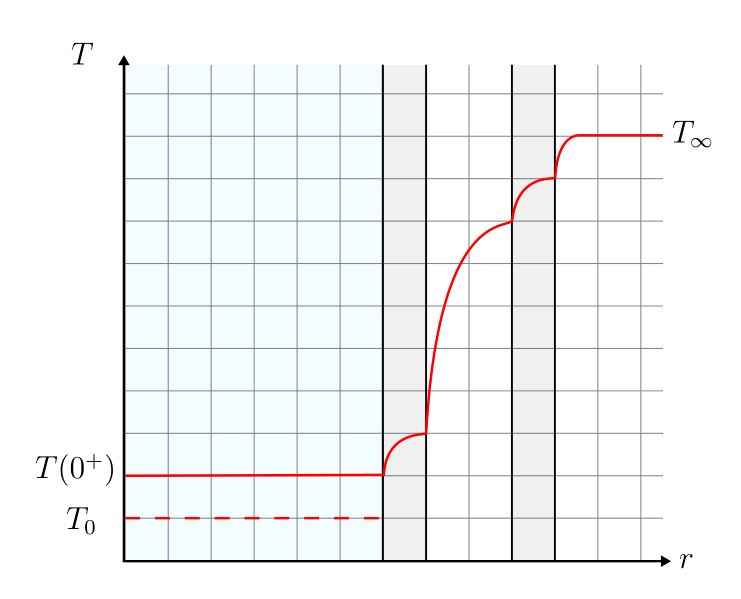
\includegraphics[width= 10cm]{tikz/15_3_2018_4a}
\end{figure}
\newline \\
b)\\ \\
Die Form des gesuchten Wärmedurchgangskoeffizienten kann der Formel \textit{Stationäre Wärmeleitung bei mehrschichtigem zylinderförmigem Wandaufbau} entnehmen und lautet somit
\[
	k(r) = \frac{1}{r}\frac{1}{\frac{1}{\lambda_w}\ln\left(\frac{r_i + w}{r_i}\right) + \frac{1}{\lambda_i}\ln\left(\frac{r_a - w}{r_i + w}\right) + \frac{1}{\lambda_w}\ln\left(\frac{r_a}{r_a - w}\right) + \frac{1}{r_a\alpha_\infty}}
\]
c)\\ \\
Die gesuchte Differentialgleichung lautet für $T(t)$
\[
	\frac{\text{d}}{\text{d}t}T(t) = -\frac{2k(r_i)}{\rho c_p r_i}(T(t) - T_\infty)
\]
d) \\ \\
Durch Lösen der obigen Differentialgleichung und einsetzen der gegebenen Bedingung erhält man die Zeit
\[
	t* = -\frac{\rho c_p r_i}{2k(r_i)}\ln\left(\frac{T* - T_\infty}{T_0 - T_\infty}\right)
\]
bei der die Flüssigkeit die gewünschte Temperatur erreicht hat.\\ \\
	\newpage	
	\subsection{17.05.2019}
	\noindent
\textbf{Beispiel 2} \\ \\
a) \\ \\

	\textbf{Beispiel 3} \\ \\
	a) \\ \\
	Der Vektor vom Ursprung zum Schwerpunkt des Rades kann direkt aus Angabe abgelesen werden und lautet deshalb:
	\begin{align*}
		\textbf{r}_r = \left[ \begin{matrix}
			p\cos\alpha - r\sin\alpha \\
			p\sin\alpha + r\cos\alpha
		\end{matrix}\right]
	\end{align*}
	Der translatorische Geschwindigkeitsvektor erhält man durch die Ableitung vom Ortsvektor nach den Freiheitsgraden.\\ \\
	Translatorischer Geschwindigkeitsvektor:
	\[
			\textbf{v}_r = \dot{\textbf{r}_r} = \left[\begin{matrix}
			\dot{p}\cos\alpha \\
			\dot{p}\sin\alpha
		\end{matrix}\right]
	\]
	Die rotatorische Geschwindigkeit lautet:
	\[ \omega_r = \frac{\dot{p}}{r}\]
	b)\\ \\
	Der Vektor zum Schwerpunkt des Stabes kann ebenfalls aus der Angabe abgelesen werden und lautet deshalb:
	\begin{align*}
		\textbf{r}_S = \left[\begin{matrix}
			p\cos\alpha - r\sin\alpha + l_s\sin\varphi \\
			p\sin\alpha + r\cos\alpha + l_s\cos\varphi
		\end{matrix}\right]
	\end{align*}
	Analog zu a) lautet der translatorische Geschwindigkeitsvektor:
	\[
		\textbf{v}_S = \dot{\textbf{r}_S} =\left[ \begin{matrix}
			\dot{p}\cos\alpha + l_s\cos\varphi\dot{\varphi} \\
			\dot{p}\sin\alpha - l_s\sin\varphi\dot{\varphi}
		\end{matrix}\right]
	\]
	\newpage
	\noindent
	c) \\ \\
	Als erstes wird die translatorische kinetische Energie des System wie folgt ermittelt:\\ \\
	Vereinfachungen:
	\begin{align*}
		\dot{\textbf{r}_r}^T\dot{\textbf{r}_r} &= \left[ \begin{matrix}
			\dot{p}\cos\alpha & \dot{p}\sin\alpha
		\end{matrix}\right]
		\left[\begin{matrix}
			\dot{p}\cos\alpha \\
			\dot{p}\sin\alpha
		\end{matrix}\right] \\
		&= \dot{p}^2\cos^2\alpha + \dot{p}^2\sin^2\alpha \\
		&= \dot{p}^2\underbrace{\left( \cos^2\alpha + \sin^2\alpha\right)}_{=1} \\
		&= \dot{p}^2 
	\end{align*}
	\begin{align*}
		\dot{\textbf{r}_S}^T\dot{\textbf{r}_S} &= \left[\begin{matrix}
		\dot{p}\cos\alpha + l_s\cos\varphi\dot{\varphi} & \dot{p}\sin\alpha - l_s\sin\varphi\dot{\varphi}
		\end{matrix}\right] \left[\begin{matrix}
		\dot{p}\cos\alpha + l_s\cos\varphi\dot{\varphi} \\
		\dot{p}\sin\alpha - l_s\sin\varphi\dot{\varphi}
		\end{matrix}\right] \\
		&=\left(\dot{p}\cos\alpha + l_s\cos\varphi\dot{\varphi}\right)^2 + \left(\dot{p}\sin\alpha + l_s\sin\varphi\dot{\varphi}\right)^2 \\
		&=\dot{p}^2\cos^2\alpha + 2l_s\dot{p}\dot{\varphi}\cos\alpha\cos\varphi + l_s^2\dot{\varphi}^2\cos^2\varphi + \dot{p}^2\sin^2\alpha - 2l_s\dot{p}\dot{\varphi}\sin\alpha\sin\varphi + l_s^2\sin^2\varphi\dot{\varphi}^2 \\
		&=\dot{p}^2\underbrace{\left(\sin^2\alpha + \cos^2\alpha\right)}_{=1} + 2l_s\dot{p}\dot{\varphi}\underbrace{\left(\cos\varphi\cos\alpha - \sin\varphi\sin\alpha\right)}_{\cos\left(\varphi + \alpha\right)} + l_s^2\dot{\varphi}^2\underbrace{\left(\sin^2\varphi + \cos^2\varphi\right)}_{=1} \\
		&= \dot{p}^2 + 2l_s\dot{p}\dot{\varphi}\cos\left(\varphi + \alpha\right) + l_s^2\dot{\varphi}^2
	\end{align*}
	Nun kann man schließlich die translatorische kinetischen Energie des Rades und des Stabes bestimmen.
	\begin{align*}
		T_{trans,r} &=  \frac{1}{2}m_r\dot{p}^2\\
		T_{trans,s} &=  \frac{1}{2}m_s\left(\dot{p}^2 + l_s^2\dot{\varphi}^2 + 2l_s\dot{p}\dot {\varphi}\cos\left(\varphi + \alpha\right)\right)
	\end{align*}
	Die kinetische Energie besitzt jedoch auch einen rotatorischen Anteil. Dieser lautet für die beiden Teilsysteme:
	\begin{align*}
		T_{rot,r} &= \frac{1}{2} \Theta_r \frac{\dot{p}^2}{r^2} \\
		T_{rot,s} &= \frac{1}{2} \Theta_s \dot{\varphi}^2
	\end{align*}
	Da wir nun sämtliche Teilenergien ermittelt haben, beträgt die gesamte kinetische Energie des vorliegenden Systems:
	\begin{align*}
		T &= T_{trans,r} + T_{rot,r} + T_{trans,s} + T_{rot,s}\\
		  &= \frac{1}{2}m_r\dot{p}^2 + \frac{1}{2} \Theta_r \frac{\dot{p}^2}{r^2} + \frac{1}{2}m_s\left(\dot{p}^2 + l_s^2\dot{\varphi}^2 + 2l_s\dot{p}\dot{\varphi}\cos\left(\varphi + \alpha\right)\right) + \frac{1}{2} \Theta_s \dot{\varphi}^2
	\end{align*}
	\newpage
	\noindent
	Als nächstes wird nun die gesamte potentielle Energie des gegebenen System ermittelt. Zuerst berechnet man wieder die Energien der Teilsysteme und addiert dieser zum Schluss wieder zusammen.
	\begin{align*}
		V_r &= m_rg\left(p\sin\alpha + r\cos\alpha\right) \\
		V_s &= m_sg\left(p\sin\alpha + r\cos\alpha + l_s\cos\varphi\right) \\
		V = V_r + V_s &= m_rg\left(p\sin\alpha + r\cos\alpha\right) + m_sg\left(p\sin\alpha + r\cos\alpha + l_s\cos\varphi\right)
	\end{align*}
	d)\\ \\
	Um den Vektor der generalisierten Kräfte zu bestimmen benötigt man zuerst den Richtungsvektor zu den Angriffspunkten der extern wirkenden Kräfte, hier $f_{ext}$. \\ \\
	Angriffspunkt der Kraft:
	\[
		\textbf{r}_f = \left[\begin{matrix}
			p\cos\alpha - r\sin\alpha + 2l_s\sin\varphi \\
			p\sin\alpha + r\cos\alpha + 2l_s\cos\varphi
		\end{matrix}\right]
	\]
	Weiters benötigt man auch den Vektor der externen Kräfte. \\ \\
	Kraftvektor:
	\[
		\textbf{f}_{ext}^T = f_{ext}\left[\begin{matrix}
			\cos\beta & \sin\beta
		\end{matrix}\right]
	\]
	Nun werden die partiellen Ableitung nach $\textbf{q}$ vom Angriffspunkt der Kraft gebildet:
	\begin{align*}
		\frac{\partial\textbf{r}_f}{\partial\varphi} = \left[\begin{matrix}
			2l_s\cos\varphi \\
			-2l_s\sin\varphi
		\end{matrix}\right] \qquad
		\frac{\partial\textbf{r}_f}{\partial p} = \left[\begin{matrix}
			\cos\alpha \\
			\sin\alpha
		\end{matrix}\right]
	\end{align*}
	Der Vektor der generalisierten Kräfte wird nun wie folgt ermittelt:
	\begin{align*}
		\textbf{f}_q = \textbf{f}_{ext}^T \frac{\partial \textbf{r}_f}{\partial \textbf{q}}
	\end{align*}
	generalisierte Kräfte:
	\begin{align*}
		f_{q,\varphi} &= f_{ext}\left[\begin{matrix}
		\cos\beta & \sin\beta
		\end{matrix}\right] \left[\begin{matrix}
		2l_s\cos\varphi \\
		-2l_s\sin\varphi
		\end{matrix}\right] \\
		&= f_{ext} \left(2l_s\cos\beta\cos\varphi - 2l_s\sin\beta\sin\varphi\right) \\
		&= f_{fext}2l_s \underbrace{\left(\cos\beta\cos\varphi - 2l_s\sin\beta\sin\varphi\right)}_{\cos\left(\beta + \varphi\right)} \\
		&= f_{ext}2l_s\cos\left(\beta + \varphi\right)
	\end{align*}
	\begin{align*}
		f_{q,p} &= f_{ext} \left[\begin{matrix}
		\cos\beta & \sin\beta
		\end{matrix}\right] \left[\begin{matrix}
			\cos\alpha \\
			\sin\alpha
		\end{matrix}\right] \\
		&= f_{ext} \underbrace{\left(\cos\beta\cos\alpha + \sin\beta\sin\alpha\right)}_{\cos\left(\beta - \alpha\right)} \\
		&= f_{ext} \cos\left(\beta - \alpha\right)
	\end{align*}
	gesamter Vektor:
	\[
		\textbf{f}_q = f_{ext} \left[\begin{matrix}
			2l_s\cos\left(\beta + \varphi\right) \\
			\cos\left(\beta - \alpha\right)
		\end{matrix}\right]
	\]
	\newpage
	\noindent
	e) \\ \\
	Zum Schluss sollen noch die Bewegungsgleichungen mithilfe des Euler-Lagrange-Formalismus bestimmt werden.
	\begin{align*}
		L &= T - V \\
		 &= \frac{1}{2}m_r\dot{p}^2 + \frac{1}{2} \Theta_r \frac{\dot{p}^2}{r^2} + \frac{1}{2}m_s\left(\dot{p}^2 + l_s^2\dot{\varphi}^2 + 2l_s\dot{p}\dot{\varphi}\cos\left(\varphi + \alpha\right)\right) + \frac{1}{2} \Theta_s \dot{\varphi}^2 \\
		 & - m_rg\left(p\sin\alpha + r\cos\alpha\right) - m_sg\left(p\sin\alpha + r\cos\alpha + l_s\cos\varphi\right)
	\end{align*}
	Bewegungsgleichungen:
	\begin{align*}
		\frac{d}{dt}\left(\frac{\partial L}{\partial \dot{\varphi}}\right) - \left(\frac{\partial L}{\partial \varphi}\right) &= 2l_sf_{ext}\cos\left(\beta + \varphi\right) \\
		\frac{d}{dt}\left(\frac{\partial L}{\partial \dot{p}}\right) - \left(\frac{\partial L}{\partial p}\right) &= f_{ext}\cos\left(\beta - \alpha\right)
	\end{align*}
	Zwischenschritte:
	\begin{align*}
		\frac{\partial L}{\partial \dot{\varphi}} &= m_s\left(l_s^2\dot{\varphi} + l_s\dot{p}\cos\left(\varphi + \alpha\right)\right) + \Theta_s \dot{\varphi} \\
		\frac{\partial L}{\partial \dot{p}} &= m_r\dot{p} + \frac{\Theta_r}{r^2}\dot{p} + m_s\left(\dot{p} + 2l_s\dot{\varphi}\cos\left(\varphi + \alpha\right)\right)
	\end{align*}
	auftretende Ableitungen:
	\begin{align*}
		\frac{\partial L}{\partial \varphi} &= -m_sl_s\sin\left(\varphi + \alpha\right)\dot{p}\dot{\varphi} + m_sgl_s\sin\varphi \\
		\frac{\partial L}{\partial p} &= -g\left(m_s + m_r\right)\sin\alpha \\
		\frac{d}{dt}\left(\frac{\partial L}{\partial \dot{\varphi}}\right) &= m_sl_s\cos\left(\varphi + \alpha\right)\ddot{p} + \left(m_sl_s^2 + \Theta_s\right)\ddot{\varphi} - m_sl_s\dot{p}\sin\left(\varphi + \alpha\right)\dot{\varphi} \\
		\frac{d}{dt}\left(\frac{\partial L}{\partial \dot{p}}\right) &= \left(m_r + \frac{\Theta_r}{r^2} + m_s\right)\ddot{p} + m_sl_s\left(\ddot{\varphi}\cos\left(\varphi + \alpha\right) - \dot{\varphi}\sin\left(\varphi + \alpha\right)\dot{\varphi} \right)
	\end{align*}
	\newpage
	\subsection{12.07.2019}
	\noindent
\textbf{Beispiel 1} \\ \\
a) \\ \\
Der Richtungsvektor vom Urspung zum Schwerpunkt der Masse $m$ lautet:
\[
	\textbf{p}_m = \left[ \begin {array}{c} r\cos \left( \alpha \right) +b
	\\ r\sin \left( \alpha \right) -h\end {array}
	\right]	
\]
Mithilfe diesen Vektor kann ebenfalls auch der Geschwindigkeitsvektor bestimmt werden, indem man den Richtungsvektor nach der Zeit ableitet.
\[
	\dot{\textbf{p}}_m =\left[ \begin {array}{c} -r \dot{\alpha}
	  \sin \left( \alpha 
	\right) + \dot{b} \\ 
	r \dot{\alpha} \cos \left( \alpha  \right) -
		\dot{h} \end {array} \right] 
\]
b) \\ \\
Um die kinetischen Energien zu berechnen, müssen zuerst einige Nebenrechnungen durchgeführt werden.\\
Nebenrechnungen:
\begin{align}
	\dot{\textbf{p}}_m^T \dot{\textbf{p}}_m &= \left[ \begin{matrix}
		-r\dot{\alpha}\sin \left( \alpha \right) + \dot{b} & r\dot{\alpha}\cos \left( \alpha \right) -\dot{h}
	\end{matrix}\right] \left[ \begin {array}{c} -r \dot{\alpha}
	\sin \left( \alpha 
	\right) + \dot{b} \\ 
	r \dot{\alpha} \cos \left( \alpha  \right) -
	\dot{h} \end {array} \right] \\
	&= r^2\dot{\alpha}^2\underbrace{\left(\cos \ \alpha  + \sin  \alpha\right)  }_{=1} -2r\dot{\alpha}\dot{b}\sin\alpha - 2r\dot{\alpha}\dot{h}\cos\alpha + \dot{b}^2 + \dot{h}^2 \\
	&= r^2\dot{\alpha}^2 -2r\dot{\alpha}\dot{b}\sin\alpha - 2r\dot{\alpha}\dot{h}\cos\alpha + \dot{b}^2 + \dot{h}^2 \\
	\varphi &= \arctan\left(\frac{h}{b}\right) \\
	\dot{\varphi} &= \frac{\dot{h}b - h\dot{b}}{b^2 + h^2}
\end{align}
kinetische Energie des Systems:
\begin{align*}
	T_{tm} &= \frac{1}{2}m\dot{\textbf{p}}_m^T \dot{\textbf{p}}_m = \frac{1}{2} m \left( r^2\dot{\alpha}^2 -2r\dot{\alpha}\dot{b}\sin\left(\alpha\right) - 2r\dot{\alpha}\dot{h}\cos\left(\alpha\right) + \dot{b}^2 + \dot{h}^2\right) \\
	T_{rm} &= \frac{1}{2} \Theta_m\dot{\varphi}^2 = \frac{1}{2} \Theta_m \left( \frac{\dot{h}b - h\dot{b}}{b^2 + h^2}\right)^2 \\
	T_{rr} &= \frac{1}{2}\Theta_r\dot{\alpha}^2 \\
	T &= T_{tm} + T_{rm} + T_{rr} \\
	  &= \frac{1}{2}m\dot{\textbf{p}}_m^T \dot{\textbf{p}}_m = \frac{1}{2} m \left( r^2\dot{\alpha}^2 -2r\dot{\alpha}\dot{b}\sin\left(\alpha\right) - 2r\dot{\alpha}\dot{h}\cos\left(\alpha\right) + \dot{b}^2 + \dot{h}^2\right) 
	  + \frac{1}{2} \Theta_m \left( \frac{\dot{h}b - h\dot{b}}{b^2 + h^2}\right)^2 + \frac{1}{2}\Theta_r\dot{\alpha}^2
\end{align*}
\newpage
\noindent
c) \\ \\
potentielle Energie des Systems:
\begin{align*}
	V_m &= mg\left(r\sin\alpha - h\right) \\
	V_c &= \frac{1}{2} c \left(\sqrt{b^2 + h^2} s_0\right)^2 \\
	V &= V_m + V_c = mg\left(r\sin\alpha - h\right) + \frac{1}{2} c \left(\sqrt{b^2 + h^2} s_0\right)^2
\end{align*}
d) \\ \\
Die viskose Reibkraft muss in der Form $f_r = \mu_V \Delta v$ beschrieben werden. In diesen Beispiel ist $\Delta v = \dot{\varphi}\textbf{r}$. \textbf{r} ist der Vektor vom Angriffspunkt der Feder zum Schwerpunkt der Masse.
\[
	\textbf{f}_V = \mu_V \underbrace{\frac{\dot{h}b - h\dot{b}}{b^2 + h^2}}_{\dot{\varphi}} \underbrace{\begin{bmatrix}
	b \\ -h
	\end{bmatrix}}_{\textbf{r}}
\]
partielle Ableitungen:
\[
	\frac{\partial \dot{\textbf{p}}_m}{\partial \alpha}  = \left[ \begin{matrix}
		-r\sin\alpha \\ r\cos\alpha
	\end{matrix}\right] \qquad \frac{\partial \dot{\textbf{p}}_m}{\partial b} = \left[ \begin{matrix}
	 1 \\ 0
	\end{matrix}\right] \qquad \frac{\partial \dot{\textbf{p}}_m}{\partial h} = \left[ \begin{matrix}
	0 \\ -1
	\end{matrix}\right]
\]
\noindent
generalisierte Kräfte:\\ \\
Multipliziert man die viskose Reibungskraft mit allen partiellen Ableitungen erhält man
\begin{align*}
	\textbf{f}_{q,v} &= \mu_V \frac{\dot{h}b - h\dot{b}}{b^2 + h^2} \left[ \begin{matrix}
		r\sin\alpha b + r\cos\alpha h \\
		-b \\
		-h
	\end{matrix}\right]
\end{align*}
Die andere externe Kraft ist
\[
	\textbf{f}_x = \left[ \begin{matrix}
		f_x \\
		0
	\end{matrix}\right]
\]
Multipliziert mit den partiellen Ableitungen erhält man
\[
	\textbf{f}_{q,x} = \left[ \begin{matrix}
		-f_x r \sin\alpha \\
		f_x \\
		0
	\end{matrix}\right]
\]
Der gesamte Vektor der generalisierten Kräfte beträgt
\[
	\textbf{f}_q = \mu_V \frac{\dot{h}b - h\dot{b}}{b^2 + h^2} \left[ \begin{matrix}
	r\sin\alpha b + r\cos\alpha h \\
	-b \\
	-h
	\end{matrix}\right] 
	+ 
	\left[ \begin{matrix}
	-f_x r \sin\alpha \\
	f_x \\
	0
	\end{matrix}\right]
\]
e) \\ \\
Verwendet man aus der Formelsammlung im Punkt generalisierte Kräfte die 2.te Formel und passt man diese an den stationären Fall an erhält man
\[
	\frac{\partial V}{\partial \textbf{q}} = \left[ \begin{matrix}
		mgr\cos\alpha\\
		\frac{c\left( \sqrt{b^2 + h^2} - s_0\right)}{\sqrt{b^2 + h^2}} b \\
		\frac{c\left( \sqrt{b^2 + h^2} - s_0\right)}{\sqrt{b^2 + h^2}} h - mg
	\end{matrix}\right]
	=
	\left[ \begin{matrix}
	-f_x r \sin\alpha \\
	f_x \\
	0
	\end{matrix}\right]
\]
Nun wird $s_0$ mit 0 angenommen und anschließend werden die generalisierten Koordinaten bestimmt. \\ \\
1.Koordinate:
\begin{align*}
	mgr\cos\alpha &= -f_xr\sin\alpha \\
	-\frac{\cos\alpha}{\sin\alpha} &= \frac{mg}{f_x}  \\
	-\tan\alpha &= \frac{mg}{f_x} \\
	\alpha &= -\arctan\left( \frac{mg}{f_x}\right)
\end{align*}
2.Koordinate:
\begin{align*}
	\frac{c\left(\cancel{\sqrt{b^2 + h^2}}\right)}{\cancel{\sqrt{b^2 + h^2}}} b &= f_x \\
	cb &= f_x \\
	b &= \frac{f_x}{c}
\end{align*}
3.Koordinate
\begin{align*}
	\frac{c\left(\cancel{\sqrt{b^2 + h^2}}\right)}{\cancel{\sqrt{b^2 + h^2}}} h -mg &= 0 \\
	ch - mg &= 0 \\
	h &= \frac{mg}{c}
\end{align*}
f) \\ \\
Die resultierende Reibkraft wird mithilfe der Formel 2.96 aus dem Vorlesungsskript berechnet und lautet hier:
\[
	\textbf{f}_F = -c_W A \frac{\rho}{2} |\dot{\textbf{p}}_m|\dot{\textbf{p}}_m
\]
\begin{align*}
	|\dot{\textbf{p}}_m| &= \sqrt{\left( -r \dot{\alpha}
		\sin \left( \alpha 
		\right) + \dot{b}\right)^2 
	+
	\left( 	r \dot{\alpha} \cos \left( \alpha  \right) -
	\dot{h}\right)^2} \\
	&= \sqrt{r^2\dot{\alpha}^2\sin^2\alpha -2r\dot{\alpha}\dot{b}\sin\alpha + \dot{b}^2 + r^2\dot{\alpha}^2\sin^2\alpha - 2r\dot{\alpha}\dot{h}\cos\alpha + \dot{h}^2} \\
	&= \sqrt{r^2\dot{\alpha}^2\underbrace{\left(\sin^2\alpha + \cos^2\alpha\right)}_{=1} - 2r\dot{\alpha}\dot{b}\sin\alpha - 2r\dot{\alpha}\dot{h}\sin\alpha + \dot{b}^2 + \dot{h}^2} \\
	&= \sqrt{r^2\dot{\alpha}^2 - 2r\dot{\alpha}\dot{b}\sin\alpha - 2r\dot{\alpha}\dot{h}\sin\alpha + \dot{b}^2 + \dot{h}^2}
\end{align*}
Multipliziert man nun $\textbf{f}_F$ mit den partiellen Ableitungen aus d) und vereinfacht man so weit wie möglich erhält man
\begin{align*}
	\textbf{f}_{q,F} &= -c_W A \frac{\rho}{2}|\dot{\textbf{p}}_m|
	\left[\begin{matrix}
		r\dot{\alpha}\underbrace{\left( \sin^2\alpha + \cos^2\alpha \right)}_{=1} - r\dot{b}\sin\alpha - r\dot{h}\cos\alpha \\
		-r\dot{\alpha}\sin \left( \alpha \right) + \dot{b} \\
		-r\dot{\alpha}\cos \left( \alpha \right) +\dot{h}
	\end{matrix}
	\right] \\
	&= -c_W A \frac{\rho}{2}|\dot{\textbf{p}}_m|
	\left[\begin{matrix}
	r\dot{\alpha} - r\dot{b}\sin\alpha - r\dot{h}\cos\alpha \\
	-r\dot{\alpha}\sin \left( \alpha \right) + \dot{b} \\
	-r\dot{\alpha}\cos \left( \alpha \right) +\dot{h}
	\end{matrix}
	\right]
\end{align*}
	\newpage
\noindent
\textbf{Beispiel 2} \\ \\
a) \\ \\
Da es sich hier um ein Problem mit Zylinderkoordinaten hält, verwendet man nun einfach die Wärmeleitgleichung für Zylinderkoordinaten aus Formelsammlung und adaptiert diese entsprechend der Angabe. \\
\newline
Wärmeleitgleichung:
\[
	0 = \lambda \left( \frac{1}{r} \frac{d}{dr}\left( \frac{d}{dr} T_i\left( r\right)\right)\right)
\]
Die 0 auf der linken Seite beruht darauf, das es sich hier um ein stationäres Problem handelt und die Terme für $\varphi$ und $z$ fallen ebenfalls weg. \\
\newline
Lösung der DGL:
\begin{align*}
	\lambda_i \left( \frac{1}{r} \frac{d}{dr}\left( r \frac{d}{dr} T_i\left( r\right)\right)\right) &= 0
	\\
	\frac{d}{dr}\left( r \frac{d}{dr} T_i\left( r\right)\right) &= 0
	\\
	\int \frac{d}{dr}\left( r \frac{d}{dr} T_i\left( r\right)\right) dr &= \int 0 dr
	\\
	r \frac{d}{dr} T_i\left( r\right) &= C_3
	\\
	\frac{d}{dr} T_i\left( r\right) &= \frac{C_3}{r}
	\\
	\int \frac{d}{dr} T_i\left( r\right) dr &= \int \frac{C_3}{r} dr
	\\
	T_i\left( r\right) &= C_3 ln\left(r \right) + C_4
\end{align*}
Randbedingungen:
\begin{align*}
	T_i\left(2R\right) &= C_3 ln\left( 2R\right) + C_4 = T_2 \\
	T_i\left(2R\right) &= C_3 ln\left( 3R\right) + C_4 = T_3
\end{align*}
Integrationskonstanten: \\
\newline
Ausgehend von dem Gleichungssystem der Randbedingung kann man die Integrationskonstanten sehr leicht bestimmen. Als ersten formt man die 2.te Gleichung auf $C_4$ um.
\begin{align*}
	T_3 &= C_3 ln\left( 3R\right) + C_4\\
	C_4 &= T_3 - C_3 ln\left( 3R\right)
\end{align*}
Dann wird in Gleichung 1 eingesetzt
\begin{align*}
	T_2 &= C_3 ln\left( 2R\right) + T_3 - C_3 ln\left( 3R\right) \\
	T_2 - T_3 &= C_3 \underbrace{\left( ln\left( 2R\right) - ln\left( 3R\right) \right)}_{ln\left( \frac{2}{3}\right)} \\
	C_3 &= \frac{T_2 - T_3}{ln\left( \frac{2}{3}\right)}
\end{align*}
Nun setzt man $C_3$ in $C_4$ ein
\begin{align*}
	C_4 &= T_3 -  \frac{T_2 - T_3}{ln\left( \frac{2}{3}\right)} ln\left( 3R\right) \\
	C_4 &= \frac{T_3 \left( ln\left( 2R\right) - ln\left( 3R\right) \right)}{ln\left( \frac{2}{3}\right)} - \frac{T_2 - T_3}{ln\left( \frac{2}{3}\right)} ln\left( 3R\right) \\
	C_4 &= \frac{T_3 ln\left( 2R \right) - T_2 ln\left( 3R\right)}{ln\left( \frac{2}{3}\right)}
\end{align*}
b) \\ \\	
Die Leistungsdichte $g$ wird wie folgt berechnet
\[
	g = \rho_e |\textbf{J}|^2 = \rho_e \left( \frac{I}{A}\right)^2
\]
mit
\[
	A = \left(4R^2 - R^2\right)\pi
\]
Dies ist die Fläche eine Hohlleiters. Setzt man nun diese in $g$ ein, erhält man
\[
	g = \rho_e \left( \frac{I}{\left(4R^2 - R^2\right)\pi}\right)^2
\]
c) \\ \\
DGL:
\begin{align*}
	\lambda_l \left( \frac{1}{r}\frac{d}{dr}\left( r\frac{d}{dr} T_l\left(r\right)\right)\right) + g = 0 \\
	\frac{d}{dr}\left( r\frac{d}{dr} T_l\left(r\right)\right) = -\frac{gr}{\lambda_l} \\
	\int \frac{d}{dr}\left( r\frac{d}{dr} T_l\left(r\right)\right) dr = \int -\frac{gr}{\lambda_l} dr \\
	 r\frac{d}{dr} T_l\left(r\right) = -\frac{gr^2}{2\lambda_l} + C_1 \\
	 \frac{d}{dr} T_l\left(r\right) = -\frac{gr}{2\lambda_l} + \frac{C_1}{r} \\
	 \int \frac{d}{dr} T_l\left(r\right) dr = \int -\frac{gr}{2\lambda_l} + \frac{C_1}{r} dr \\
	 T_l\left(r\right) = -\frac{gr^2}{4\lambda_l} + C_1\ln\left( r \right) + C_2
\end{align*}
Randbedingungen
\begin{align*}
	T_l\left(R\right) = -\frac{gR^2}{4\lambda_l} + C_1\ln\left(R\right) + C_2 = T_1 \\
	T_l\left(2R\right) = -\frac{g4R^2}{4\lambda_l} + C_1 \ln\left(2R\right) + C_2 = T_2
\end{align*}
\newpage
\noindent
Integrationskonstanten: \\ \\
Die beiden Konstanten werden wie in a) bestimmt.
\begin{align*}
	-\frac{gR^2}{4\lambda_l} + C_1\ln\left(R\right) + C_2 = T_1 \\
	C_2 = T_1 + \frac{gR^2}{4\lambda_l} - C_1\ln\left(R\right)
\end{align*}
Diese Gleichung wird nun in die andere eingesetzt und man erhält
\begin{align*}
	-\frac{g4R^2}{4\lambda_l} + C_1 \ln\left(2R\right) + T_1 + \frac{gR^2}{4\lambda_l} - C_1\ln\left(R\right) = T_2 \\
	\frac{g}{4\lambda_l}\left(R^2 - 4R^2\right) 
	+ T_1 - T_2 = C_1 \underbrace{\left( ln\ln\left(1\right) - \ln\left(2\right)\right)}_{\ln\left( \frac{1}{2}\right)} \\
	C_1 = \frac{\frac{g}{4\lambda_l}\left(R^2 - 4R^2\right) + T_1 - T_2}{\ln\left( \frac{1}{2}\right)}
\end{align*}
Rückeingesetzt erhält man
\begin{align*}
	C_2 &= T_1 + \frac{gR^2}{4\lambda_l} - \frac{\frac{g}{4\lambda_l}\left(R^2 - 4R^2\right) + T_1 - T_2}{\ln\left( \frac{1}{2}\right)}\ln\left(R\right) \\
	&= \frac{T_1\left(\ln\left(R\right) - \ln\left(2R\right)\right)}{ln\left(\frac{1}{2}\right)} + 
	\frac{\frac{gR^2}{4\lambda_l}\left(\ln\left(R\right) - \ln\left(2R\right)\right)}{\ln\left( \frac{1}{2}\right)} \\
	&- \frac{\frac{g}{4\lambda_l}\left(R^2\ln\left(R\right) - 4R^2\ln\left(R\right)\right) + T_1\ln\left(R\right) - T_2\ln\left(R\right)}{\ln\left( \frac{1}{2}\right)} \\
	&= \frac{\frac{g}{4\lambda_l}\left(4R^2\ln\left(R\right) - R^2\ln\left(2R\right)\right) + T_2\ln\left(R\right) - T_1\ln\left(2R\right)}{\ln\left(\frac{1}{2}\right)}
\end{align*}
d) \\ \\
Zur eindeutigen Bestimmung der Temperaturen \(T_1 , T_2 , T_3\) muss einfach nur die Gleichungen für die Wärmeübergänge aufstellen. Diese lauten für \\ \\
\(T_2:\)
\[
	\lambda_i\frac{d}{dr}T_i\left(r\right)|_{r = 2R} = \lambda_l \frac{d}{dr}T_l\left(r\right)|_{r = 2R}
\]
\(T_3:\)
\[
	\alpha_0\left(T_\infty - T_3\right) = \lambda_i\frac{d}{dr}T_i\left(r\right)|_{r = 3R}
\]
\(T_1:\)
\[
	\alpha_f\left(T_f - T_1\right) = -\lambda_l\frac{d}{dr}T_l\left(r\right)|_{r = R}
\]
\newpage
\noindent
e) \\ \\
1) Temperatur der Kühlflüssigkeit senken \\
2) Oberfläche der Isolierung vergrößern (z.B. durch Kühlrippen) \\
3) Wärmeleitfähigkeit der Isolierung vergrößern \\
\\
\textit{Hinweis}:\\
\textit{Die Lösung in diesen Punkt erhält man durch logisch denken.}

	\newpage
\noindent
\textbf{Beispiel 3} \\ \\
a)
\vspace{-15pt}
\usetikzlibrary{arrows}
\begin{figure}[h]
	\centering
\begin{tikzpicture}
\draw (-3.5,-1) -- (-3.5,-2) -- (-2,-2) -- (-2,-1) -- (-3.5,-1);
\draw (-2.75,-1) -- (-2.75,0.5);
\draw [-latex][red,very thick](-2.75,0.0232) -- (-2.75,1.0);
\draw[-latex][red,very thick](-2.75,-0.5) -- (-2.75, -1.5);
\draw (-2.3377,-1.4121) node {\( mg\)} ;
\draw (-2.228,0.8364) node {\( F_{s,1}\)};
\draw (-1.62,5.145) -- (-0.3,4.2);
\draw  (-2,4.5) circle (0.75);
\draw (-2.75,4.5) -- (-2.75,3.5);
\draw [-latex][red,very thick](-2.75,3.5) -- (-2.75,2.5);
\draw [-latex][red,very thick] (-3,4.5) -- (-2,4.5);
\draw [latex-][red,very thick]  (-2,4.5) -- (-2,6);
\draw [latex-][red,very thick]  (-2,4.5) -- (-2,3);
\draw [-latex][red,very thick](-1.8834,3.8167) arc (-67.5126:26.8608:0.8);
\node at (-2.2741,2.505) {\(F_{s,1}\)};
\node at (-1.6074,3.205) {\( F_{E,y}\)};
\node at (-3.249,4.755) {\(F_{E,x}\)};
\node at (-1.6074,5.755) {\(m_sg\)};
\node at (-1.6574,4.5217) {\( \tau\)};
\draw [-latex][red,very thick] (-0.3,4.2) --(0.5,3.6);
\node at (0.5,4) {\( F_{s,2}\)};
\draw [latex-][red,very thick](0.8,3.4) -- (1.5,2.9);
\draw (1.5,2.9) -- (2.2,2.4);
\node at (1.2,3.5) {\(F_{s,2}\)};
\node at (2.3,2.2) {Lager};
\end{tikzpicture}
\end{figure}
\\ 
Nun müssen die Gleichgewichtsbedingungen für diesen Schnitt bestimmt werden. Diese lauten hier
\begin{align*}
	&\sum M_E = 0: \\
	&\tau -F_{s,2}r + F_{s,1}r = 0 \\
	\\
	&\sum F_x = 0: \\
	&F_{E,x} + F_{s,2}\sin\left(\frac{\pi}{4}\right) = 0 \\
	&F_{E,x} + \frac{F_{s,}}{\sqrt{2}}= 0 \\
	\\
	&\sum F_y = 0:\\
	&F_{E,y} - F_{s,1} - F_{s,2}\sin\left(\frac{\pi}{4}\right) - m_sg = 0\\
	&F_{E,y} - F_{s,1} - \frac{F_{s,2}}{\sqrt{2}} - m_sg = 0
\end{align*}
\newpage
Nun werden die Kräfte im Punkt E und die Seilkräfte berechnet.
\begin{align*}
	&F_{s,1} = mg \\
	\\
	&\tau -F_{s,2}r + F_{s,1}r = 0 \\
	& F_{s,2} r = \tau + m g r \\
	& F_{s,2} = mg + \frac{\tau}{r} \\
	\\
	&F_{E,x} + \frac{F_{s,2}}{\sqrt{2}}= 0 \\
	&F_{E,x} + \frac{mg}{\sqrt{2}} + \frac{\tau}{r\sqrt{2}} = 0 \\
	&F_{E,x} = - \frac{mg}{\sqrt{2}} - \frac{\tau}{r\sqrt{2}} \\
	\\
	&F_{E,y} - F_{s,1} - \frac{F_{s,2}}{\sqrt{2}} - m_sg = 0 \\
	&F_{E,y} - mg - \frac{mg}{\sqrt{2}} - \frac{\tau}{r\sqrt{2}} - m_sg = 0 \\
	&F_{E,y} = mg \frac{\sqrt{2} + 1}{\sqrt{2}} + \frac{\tau}{r\sqrt{2}} + m_sg
\end{align*}
b)
\begin{figure}[h]
	\centering
\begin{tikzpicture}[scale = 1.5]
\draw (-0.5,0.5) -- (-2,1.5) -- (-0.5,1.5);
\draw [red,very thick][-latex](-3.5,1.5) -- (-2,1.5);
\node at (-3.5,1) {\( F_{B,x}\)};
\draw (-2,1.5) -- (-2,-2.5) -- (-0.5,-2.5);
\draw [red,very thick][-latex](-2,0) -- (-2,1.5); 
\node at (-1.5,0.5) {\(F_{B,y}\)};
\draw [red,very thick][-latex](-3.5,-2.5) -- (-2,-2.5);
\node at (-3.5,-2) {\(F_A\)};
\end{tikzpicture}
\end{figure}
\newpage
Nun werden analog wie in a) die Gleichgewichtsbedingungen aufgestellt.
\begin{align*}
	&\sum M_A = 0: \\
	& F_{B,x}h + F_{E,y} \left(a + b\right) -fa = 0 \\
	& F_{B,x} = - F_{E,y}\frac{a+b}{h} + f\frac{a}{h} \\%Fehler in der Musterlösung
	\\
	&\sum F_x = 0:\\
	&F_{B,x} + F_A +F_{E,x} = 0\\
	&-F_{E,y}\frac{a + b}{h} + f \frac{a}{h} + F_A + F_{E,x} = 0 \\
	&F_A = F_{E,y}\frac{a + b}{h} - f\frac{a}{h} - F_{E,x}  \\
	\\
	&\sum F_y = 0: \\
	&F_{B,y} + F_{E,y} - f = 0 \\
	&F_{B,y} = f - F_{E,y}
\end{align*}
\textbf{ACHTUNG}: Die Ergebnisse in der Musterlösung vom ACIN sind nicht korrekt.\\ \\
c)
\begin{figure}[h]
\centering
\begin{tikzpicture}[scale = 1.5]
\draw (-0.5,0.5) -- (-2,1.5) -- (-0.5,1.5);
\draw [red,very thick][-latex](-3.5,1.5) -- (-2,1.5);
\node at (-3.5,1) {\( F_{B,x}\)};
\draw [blue,very thin](-2,1.5) -- (1.5,1.5);
\draw [blue,very thin](-2,1.5) -- (0.7,-0.3);
\draw [blue,thick][latex-latex](0.4,-0.1) arc (-33.5006:0:2.9);
\node at (1.1,0.6) {\(\alpha\)};
\draw (-2,1.5) -- (-2,-2.5) -- (-0.5,-2.5);
\draw [red,very thick][-latex](-2,0) -- (-2,1.5); 
\node at (-1.5,0.5) {\(F_{B,y}\)};
\draw [red,very thick][-latex](-3.5,-2.5) -- (-2,-2.5);
\node at (-3.5,-2) {\(F_A\)};
\draw [red,very thick][-latex](-1,-2.5) -- (0.5,-2.5);
\node at (-0.5,-2) {\(F_2\)};
\draw [red,very thick][-latex](-1,1.5) -- (0,1.5);
\node at (-0.5,2) {\(F_4\)};
\draw [red,very thick][-latex](-0.8,0.7) -- (-0.2,0.3);
\node at (0,0.5) {\(F_3\)};
\end{tikzpicture}
\end{figure}
\newpage
Es müssen wieder die Gleichgewichtsbedingungen aufgestellt werden. Diese lauten hier
\begin{align*}
	&\alpha = \arctan\left(\frac{h}{a}\right) \\
	&\sum M_B = 0: \\
	&F_Aa + F_2 a = 0 \\
	&F_2 = -F_A \\
	\\
	&\sum F_y = 0: \\
	&F_{B,y} - F_3 \sin\alpha = 0 \\
	&F_3 = \frac{F_{B,y}}{\sin\alpha} \\
	\\
	&\sum F_x = 0: \\
	&F_2 + F_4 + F_3 \cos\alpha + F_{E,x}= 0 \\
	&F_4 = - F_2 - F_{B,y}\frac{\cos\alpha}{\sin\alpha} - F_{E,x}\\
	&F_4 = F_A - \frac{F_{B,y}}{\tan\alpha} - F_{E,x}
\end{align*}
	\newpage
\noindent
\textbf{Beispiel 4} \\ \\
a) \\ \\
Die zu berechnenden Wärmestromdichten können mit der Formel für Konvektion aus der Formelsammlung des ACIN bestimmt werden. Diese lauten
\begin{align*}
	&\dot{q}_O = \alpha_O \left(T_M - T_L\right) , \qquad \dot{q}_{L,2} = \alpha_L \left(T_2 - T_L\right) \\
	&\dot{q}_M = \alpha_M \left(T_M - T_1\right) , \qquad \dot{q}_{L,3} = \alpha_L \left(T_3 - T_L\right) \\
	&\dot{q}_B = \alpha_B \left(T_4 - T_B\right)
\end{align*}
Bei den Ausdrücken, wo laut Formel sich eigentlich ein \(-\) ergibt, wird das Vorzeichen vertauscht, damit keine negativen Wärmestromdichten mehr vorkommen. \\ \\
b) \\ \\
Nun soll die Sichtfaktormatrix \(\textbf{F}\) bestimmt werden.\\
Bestimmung der einzelnen Einträge von \(\textbf{F}\):
\[
	F_{11} = F_{44} = 0
\]
Wand 1 und 4 strahlen thermisch nicht auf sich selbst. Die anderen Einträge der Hauptdiagonalen können mit der Tabelle auf Seite 5 der Formelsammlung des ACIN ermittelt werden und lauten deswegen
\begin{align*}
	F_{22} = F_{33} = 1 -\frac{\sqrt{1^2+2^2}}{1+2} = \frac{3 - \sqrt{5}}{3}
\end{align*}
Die restlichen Einträge werden entweder mit der Cross-String-Methode, dem Reziprozitätsgesetz, der Summationsregel oder durch Symmetrie des Aufbaues ermittelt.
\begin{align*}
	&F_{24} = F_{34} = \frac{3 + \sqrt{5} - \left(1 + \sqrt{5}\right)}{2\cdot3} = \frac{2}{2 \cdot 3} = \frac{1}{3} \\
	&F_{42} = F_{43} = \frac{A_2}{A_4}F_{24} = \frac{3}{3} \frac{1}{3} = \frac{1}{3} \\
	&F_{41} = 1 - F_{42} - F_{43} - F_{44} = 1 - \frac{1}{3} - \frac{1}{3} - 0 = \frac{1}{3} \\
	&F_{14} = \frac{A_4}{A_1}F_{41} = \frac{3}{3} \cdot \frac{1}{3} = \frac{1}{3} \\
	&F_{12} = F_{13} = \frac{\sqrt{5} + 3 - \left(1 - \sqrt{5}\right)}{2\cdot 3} = \frac{2}{2 \cdot 3} = \frac{1}{3} \\
	&F_{21} = F_{31} = \frac{A_1}{A_2}F_{12} = \frac{3}{3}\cdot \frac{1}{3} = \frac{1}{3} \\
	&F_{23} = 1 - F_{21} - F_{22} - F_{24} = 1 - \frac{1}{3} -\frac{3 - \sqrt{5}}{3} - \frac{1}{3} = \frac{\sqrt{5} - 2}{3} \\
	&F_{32} = \frac{A_2}{A_3}F_{23} = \frac{3}{3} \cdot \frac{\sqrt{5} - 2}{3} = \frac{\sqrt{5} - 2}{3}
\end{align*}
\newpage
\noindent
Die komplette Sichtfaktormatrix lautet
\[
	\textbf{F} = \left[\begin{matrix}
	0 & \frac{1}{3} & \frac{1}{3} & \frac{1}{3} \\
	\frac{1}{3} & \frac{3 - \sqrt{5}}{3} & \frac{\sqrt{5} - 2}{3} & \frac{1}{3} \\
	\frac{1}{3} & \frac{\sqrt{5} - 2}{3} & \frac{3 - \sqrt{5}}{3} & \frac{1}{3} \\
	\frac{1}{3} & \frac{1}{3} & \frac{1}{3} & 0
	\end{matrix}\right]
\]
c) \\ \\
Die folgenden Ausdrücke kann man einfach aus der Formelsammlung herauslesen. 
\begin{align*}
	\dot{\textbf{q}} = \left[\begin{matrix}
		\dot{\textbf{q}}_M \\
		-\dot{\textbf{q}}_{L,2} \\
		-\dot{\textbf{q}}_{L,3} \\
		-\dot{\textbf{q}}_B
	\end{matrix}\right]
	\qquad
	\textbf{T}^4 = \left[\begin{matrix}
		T_1^4 \\
		T_2^4 \\
		T_3^4 \\
		T_4^4
	\end{matrix}\right]
	\qquad
	\varepsilon = \left[\begin{matrix}
		\varepsilon \\
		\varepsilon \\
		\varepsilon \\
		\varepsilon
	\end{matrix}\right] \\
	\textbf{P} = diag\{\varepsilon\}\left(\textbf{E} - \left(\textbf{E} - diag\{\varepsilon\}\right)^{-1}\right)\left(\textbf{E}-\textbf{F}\right)\sigma\textbf{T}^4
\end{align*}
d) \\ \\
Die Differentialgleichung für den Zeitverlauf von \(T_M\left(t\right)\) lautet
\[
	1m^2\rho c_p \frac{dT_M\left(t\right)}{dt} = -1m\underbrace{\alpha_O\left(T_M\left(t\right) - T_L\left(t\right)\right)}_{\dot{q}_O} -3m\dot{q}_M\left(T_M\left(t\right),T_B\left(t\right),T_L\left(t\right)\right)
\]
Die Unbekannten sind \(\dot{q}_O,\dot{q}_M,\dot{q}_{L,2},\dot{q}_{L,3},T_1,T_2,T_3,T_4\), die alle durch Umformen der Gleichung von a) und c) berechnet werden können. \\ \\
e) \\ \\
Nun kann laut Formelsammlung die Gleichung aus d) diskretisiert werden.
\[
	t_k = k\Delta t
\]
\[
	1m^2\rho c_p \frac{T_M\left(t_{k+1}\right) - T_M\left(t_k\right)}{\Delta t} = -1m\alpha_O\left(T_M\left(t_k\right) - T_L\left(t_k\right)\right) -3m\dot{q}_M\left(T_M\left(t_k\right),T_B\left(t_k\right),T_L\left(t_k\right)\right)
\]
	\newpage
	\subsection{27.09.2019}
	\subsection{08.11.2019}
\end{document}